\chapter{Story Lane Theater - Overview}

Story Lane Theater is a series of videos originally produced by Rabbit Ears Productions, but which were then later re-released by The Lightspan Partnership for the PlayStation. There are five CDs in total, with each CD containing two videos, for a total of ten videos in the series. Each of the videos in the series is designed to give a brief overview of classic children's story, including stories from outside the United States.

Although there are other series produced by Lightspan that only feature a variety of videos, what is interesting about Story Lane Theater is that all of their content is licensed from Rabbit Ears Productions.

Rabbit Ears Productions was formed in 1984, but released their first video, "The Velveteen Rabbit", in 1985 on public television, before eventually releasing their later videos on VHS. Throughout the company's existence, it produced a large number of television episodes, with each episode featuring a celebrity narrator, and a musical score by a well-known composer, and were animated by a variety of different animators. The company was eventually dissolved in 1997, but their videos have since been re-released on DVD.

\begin{figure}[H]
    \centering
    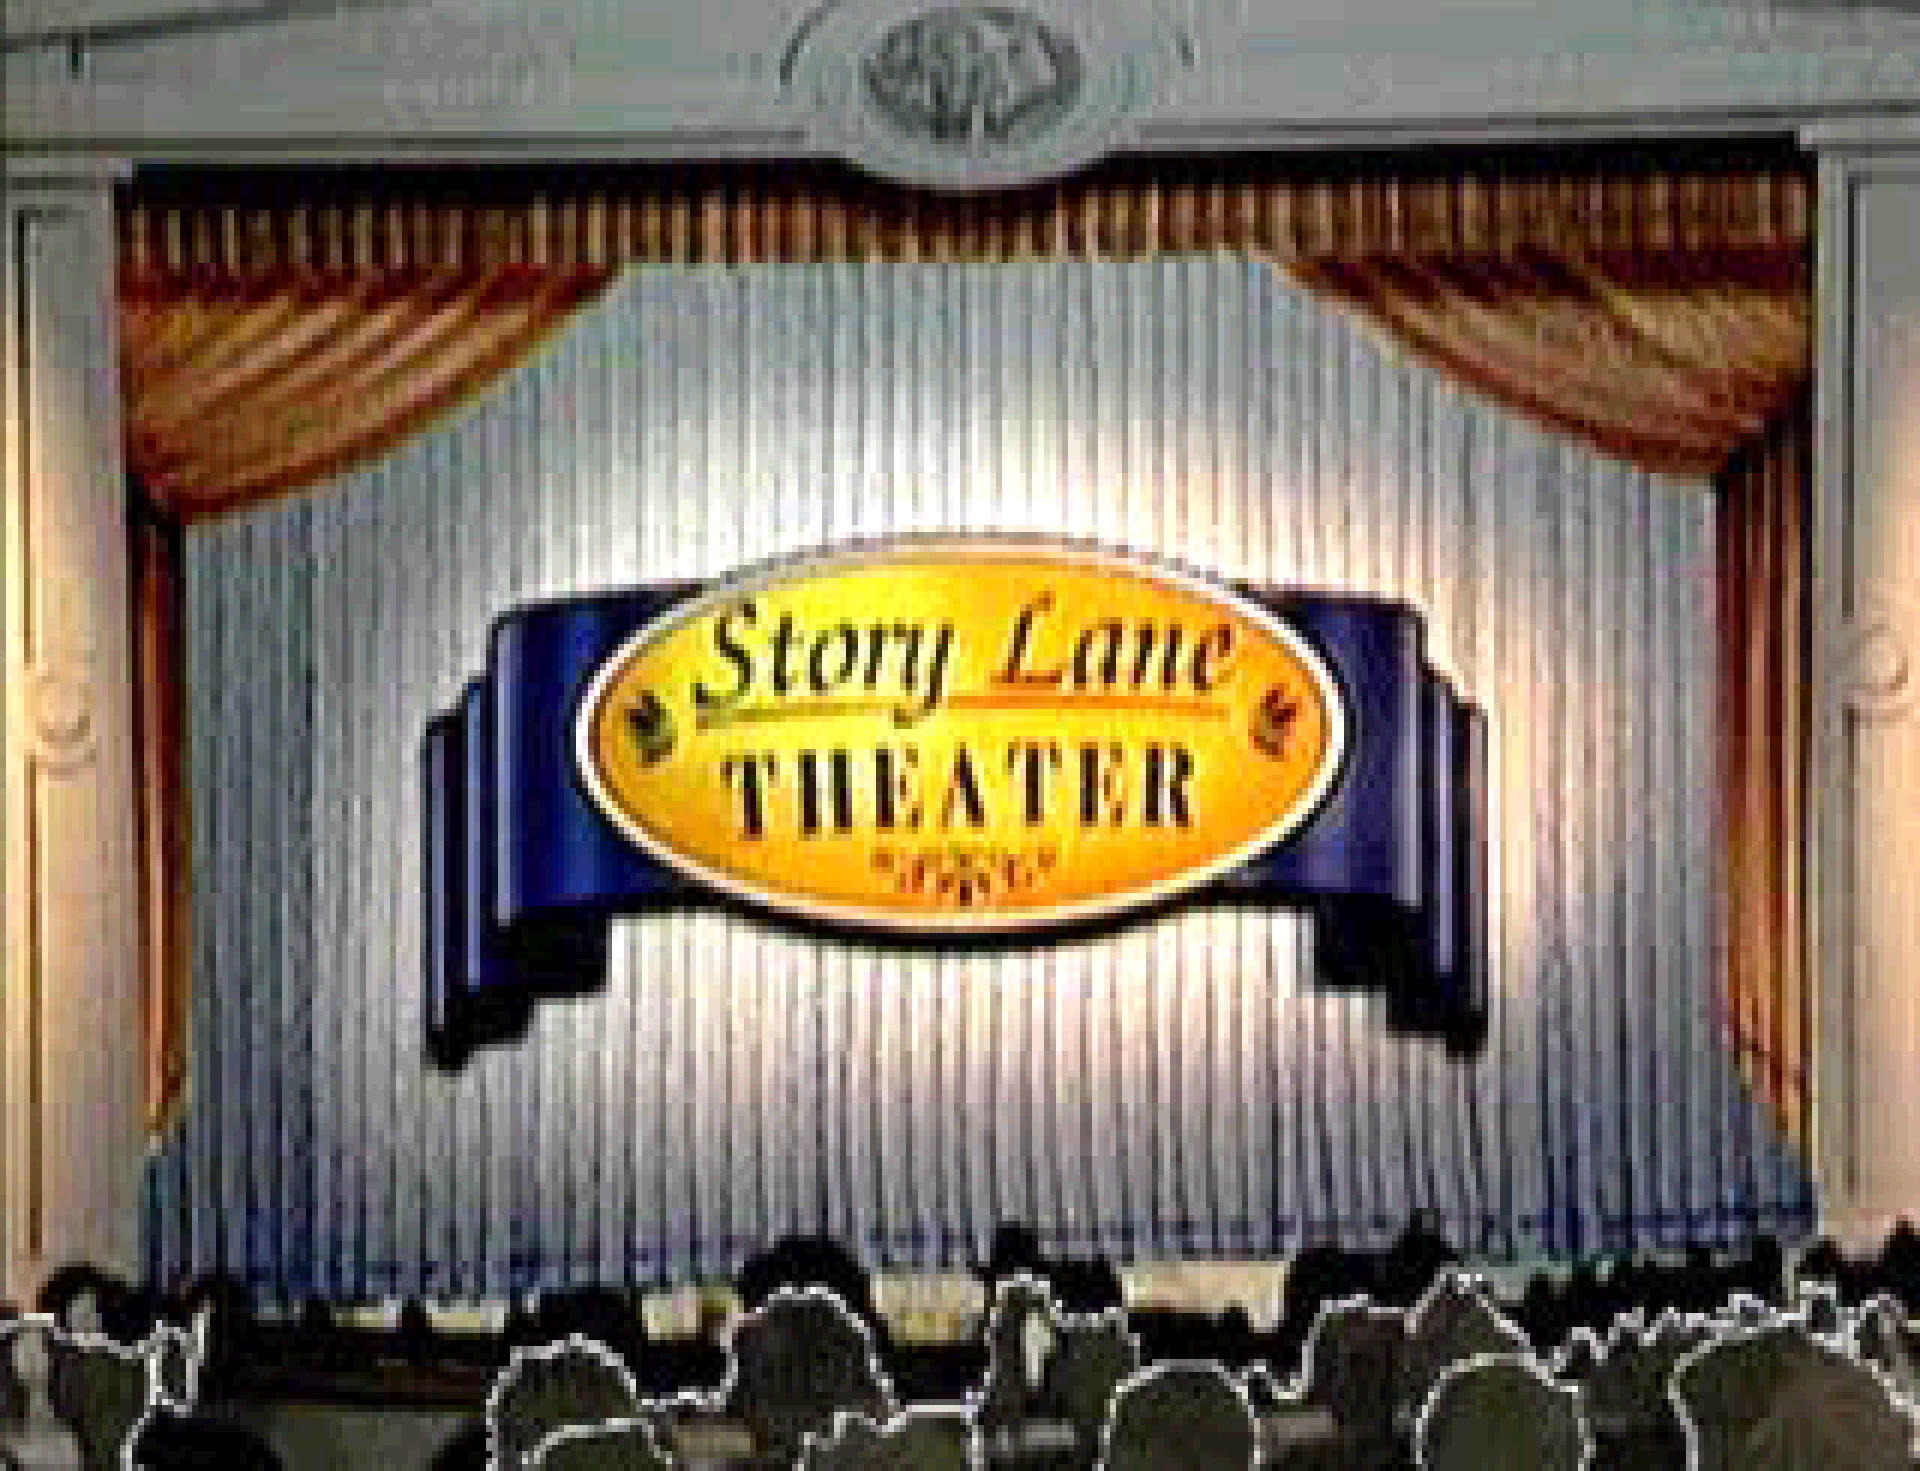
\includegraphics[width=0.5\textwidth]{./Games/StoryLaneTheater/Images/StoryLaneTheaterMainImage.png}
    \caption{Story Lane Theater Logo}
\end{figure}

When the Story Lane Theater were re-released by Lightspan, one of the primary differences that were included with these were that each of the stories now contained a "Backstage Pass" documentary, which featured interviews with the celebrities who narrated the stories, as well as the animators who worked on the videos. For the most part, these documentaries are fairly short, and are usually only a few minutes long. However, to the best of my knowledge, these documentaries were not included in most of the original Rabbit Ears Productions releases.

In addition to this, the title sequence for each of the videos was also changed, with the original Rabbit Ears Productions title sequence being replaced with a new one that was created by Lightspan featuring the curtain opening on a number of companies, including Macmillain/McGraw-Hill School Division, Rabbit Ears Productions, and Story Lane Theater, which appears to be what Rabbit Ears called the series when they re-released the videos for the PlayStation, as well as on VHS.

Apart from the Wikipedia page for Rabbit Ears Productions, there is very little information available about the company and the list of productions produced. The company produced 65 episodes in total, spanning four seasons, with their final episodes being released in 1994. The company was then purchased at some point by Vanguard Animation, an production studio kwnown for a number of 3D animated films including Space Chimps and Gnome Alone. At a later stage, Penguin Random House have made many of the stories available as audiobooks through their Listening Library service.